\subsection{Oportunidades para uso da constru\c c\~{a}o \texttt{multi-catch}}

O mecanismo de tratamento de exceção sempre esteve 
presente na linguagem Java; entretanto, Java 7 forneceu uma 
evolução elegante e que permite ao desenvolvedor utilizar blocos \texttt{multi-catch} que possibilitam 
a concatenação de \texttt{catchs} iguais ou similares. Com isso, a adoção deste 
recurso permite a redução da lógica duplicada 
em \texttt{catchs} distintos de uma mesma construção \texttt{try-catch}.

Com as análises realizadas, foi possível identificar uma quantidade significativa de oportunidades 
de uso dessa construção, conforme exibido na Figura:~\ref{fig:Muticatch}. Ao todo \num{95}\% dos projetos pesquisados possuem oportunidades reais para aplicação de \texttt{multi-catch} e
foram encontrados \num{1474} blocos \texttt{try} que possuem \textit{catchs} repetidos. 
Estas ocorrências estão distribuídas em \num{1028} arquivos e totalizando \num{30936} \acs{LOC}. 
Importante observar que o teste de  similaridade entre os blocos \texttt{catch} 
foi realizado através de uma chamada a um método externo que verifica a igualdade da árvore 
sintática. Apesar dessa abordagem não fazer uso de uma estratégia de análise 
de similaridade de código mais robusta, a mesma pode ser facilmente alterada de 
acordo com algum algoritmo existente. A Tabela:~\ref{tab:oportunidadesMulticatch} exibe a distribuição de oportunidades de \texttt{multi-catch} pela natureza do sistema.

\begin{figure}[h]
	\center
	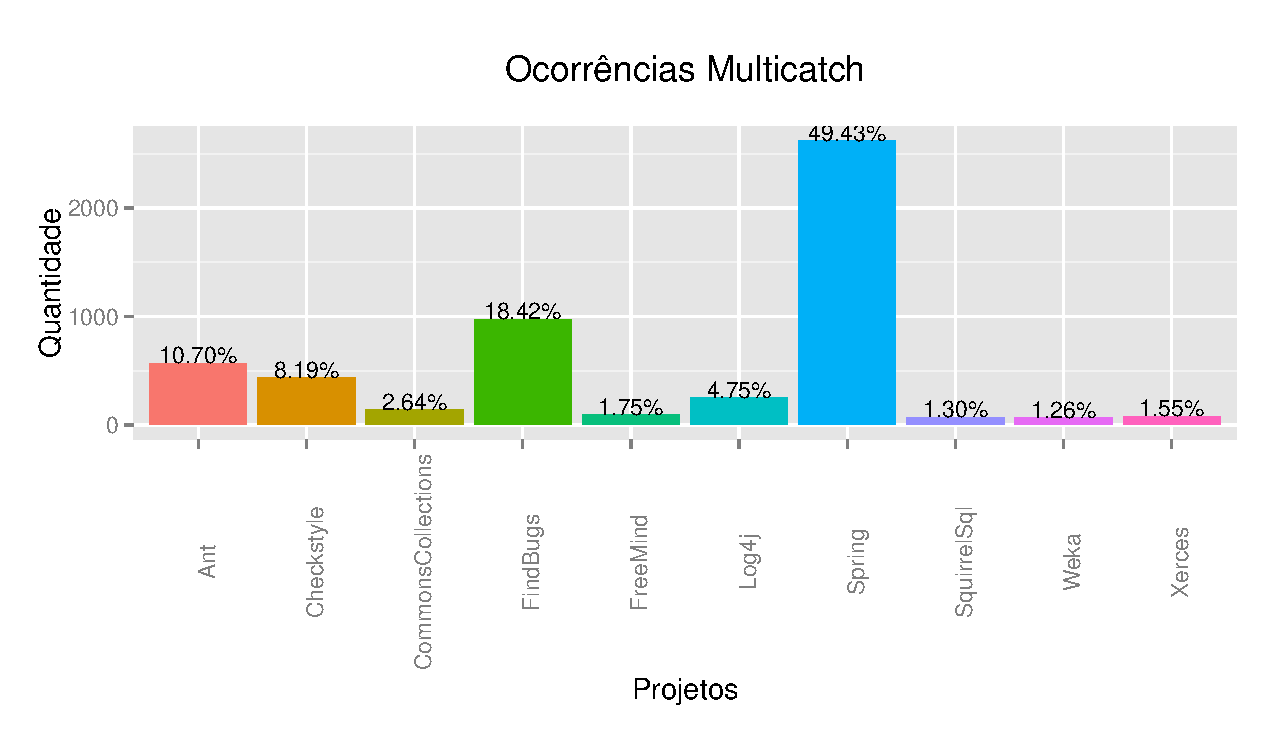
\includegraphics[scale=0.75]{Imagens/ocorrenciasMulticatch}
	\label{fig:Muticatch}
	\caption{Oportunidades de \texttt{multi-catch} nos projetos.}
\end{figure}
	
\begin{table}[h]
	\centering
	\caption{Oportunidades de \texttt{multi-catch} por tipo do sistema.}
	\begin{tabular}{cc}
		\hline
		Natureza & Ocorrências \\ 
		\hline \hline
		\texttt{Application} & 551 \\ 
		\texttt{Library} &  464 \\ 
		\texttt{Servers - Database} &  459 \\ \hline
		\texttt{Total} &  1474 \\ \hline
	\end{tabular}
	\label{tab:oportunidadesMulticatch} %std means summary of type declarations
\end{table}
		
A implantação de \texttt{multi-catch} em um projeto pode ser iniciada com substituição de blocos \texttt{catch} aninhados por este recurso tornado evidente a redução significativa das ~\acs{LOC} duplicadas. A classe \texttt{AbstractNestablePropertyAccessor} do projeto  \textit{Spring 4.2.0.RC2} contém \texttt{catch} duplicado conforme a listagem:~\ref{lst:semMulticatch}. Entretanto após um \textit{refactoring} na Listing:~\ref{lst:semMulticatch} para implantação do recurso \texttt{multi-catch} pode-se verificar na Listing:~\ref{lst:comMulticatch} a redução significativa de código duplicado na ordem de \num{42}\% o que torna este recurso muito útil sem causar grandes mudanças no software.


%Considere os exemplos nas listagens:~\ref{lst:codigoSemMulticatch} e ~\ref{lst:codigoComMulticatch}, 
%encontrados na classe \texttt{AbstractNestablePropertyAccessor} do projeto \textit{Spring 4.2.0.RC2}. 
%Neste caso, é possível reestruturar o c\'{o}digo para usar a constru\c c\~{a}o 
%\texttt{multi-catch}, o que levaria a uma redu\c c\~{a}o de {\color{red} 40\%}  para 
%esse trecho de código. Um simples \textit{refactoring} unindo todos os blocos 
%que potencialmente se beneficiariam do uso de blocos \texttt{multi-catch} levaria a uma redução de 
%68063 \acs{LOC}, tornando essa constru\c c\~{a}o  \'{u}til para reduzir a quantidade de 
%linhas de c\'{o}digo em duplicidade de um projeto. 
\begin{lstlisting}[caption={Código sem adoção de multi-catch}\label{lst:semMulticatch},language=Java] 
try {
	...
}catch (ConverterNotFoundException ex) {
  PropertyChangeEvent pce = new PropertyChangeEvent(this.rootObject, this.nestedPath + propertyName, oldValue, newValue);
  throw new ConversionNotSupportedException(pce, td.getType(), ex);
}catch (ConversionException ex) {
  PropertyChangeEvent pce = new PropertyChangeEvent(this.rootObject, this.nestedPath + propertyName, oldValue, newValue);
  throw new TypeMismatchException(pce, requiredType, ex);
}catch (IllegalStateException ex) {
  PropertyChangeEvent pce = new PropertyChangeEvent(this.rootObject, this.nestedPath + propertyName, oldValue, newValue);
  throw new ConversionNotSupportedException(pce, requiredType, ex);
}catch (IllegalArgumentException ex) {
  PropertyChangeEvent pce = new PropertyChangeEvent(this.rootObject, this.nestedPath + propertyName, oldValue, newValue);
  throw new TypeMismatchException(pce, requiredType, ex);
}
\end{lstlisting}


\begin{lstlisting}[caption={Refactoring com uso de multi-catch}\label{lst:comMulticatch},language=Java] 
 try {
	 ...
 } catch (ConverterNotFoundException ex | IllegalStateException ex) {
   PropertyChangeEvent pce = new PropertyChangeEvent(this.rootObject, this.nestedPath + propertyName, oldValue, newValue);
   throw new ConversionNotSupportedException(pce, td.getType(), ex);
 }catch (ConversionException ex | IllegalArgumentException ex) {
   PropertyChangeEvent pce = new PropertyChangeEvent(this.rootObject, this.nestedPath + propertyName, oldValue, newValue);
   throw new TypeMismatchException(pce, requiredType, ex);
 }	
\end{lstlisting}

%Foi levantado junto a comunidade a não adoção desta característica da linguagem devido sua simplicidade de implantação e redução de código duplicado e a resposta obtida foi: \textcolor{red}{resposta da comunidade. + (link).}


%Uma análise mais detalhada sobre \textit{JBoss, Spring, Hibernate e Findbugs} totalizando juntos 7778 ocorrências, iniciando na 3.0.0.M1 lançada em junho de 2009 até a mais recente até o momento 4.2.0.RC2. Para uma análise mais criteriosa será elaborada um detalhamento a partir da versão 4.0.0.M1 até a 4.2.0.RC2 totalizando 927 oportunidades de \textit{multicatch} 35\% das ocorrências no \textit{Spring}.\\

%A figura: \ref{fig:ocorrenciasMulticatchVersoes} exibe as ocorrências nos projetos mais numerosos do estudo. Onde todas as ocorrências totalizam 17100 \acs{LOC} e após um simples \textit{refactoring} conforme demonstrado nos listagens:~\ref{lst:semMulticatch} e ~\ref{lst:comMulticatch}, obtem-se 5955 \acs{LOC} o que acarreta uma redução  de \num{65}\% de código duplicado em blocos \texttt{catch}.

%\begin{figure}[h]
%	\center
%	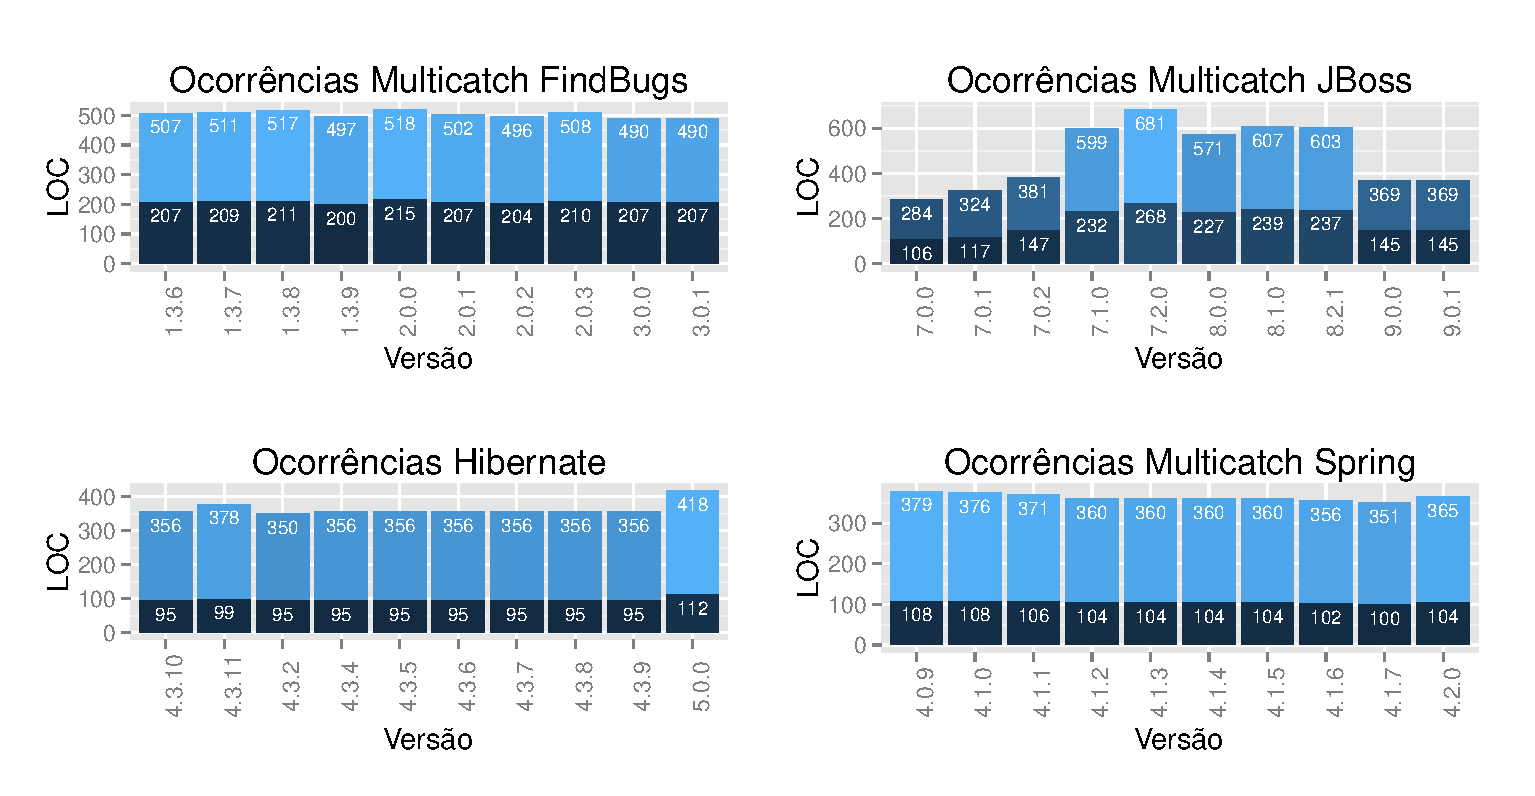
\includegraphics[height=8cm, keepaspectratio]{Imagens/ocorrenciasMulticatchVersoes}
%	\label{fig:ocorrenciasMulticatchVersoes}
%	\caption{Oportunidades de \textit{Multicatch} nos projetos.}
%\end{figure}

